\documentclass[a4paper, 14pt]{extarticle}
\usepackage[top=1in, bottom=1in, left=1in, right=1in]{geometry}
\usepackage{amsmath}
\usepackage{amssymb}
\usepackage{graphicx}
\usepackage{hyperref}
\usepackage{tcolorbox}
\usepackage{tikz}
\usepackage{tikz-3dplot}
\usepackage{fontspec}
%\usetikzlibrary{decorations.pathmorphing}
\usetikzlibrary{calc,decorations,patterns,arrows,decorations.pathmorphing,3d}
\definecolor{pltblue}{HTML}{1F77B4}
\tikzset{every picture/.style={/utils/exec={\fontspec{Humor Sans}}}}
\setmainfont{Pretty Neat}

\makeatletter
\pgfset{
  /pgf/decoration/randomness/.initial=2,
  /pgf/decoration/wavelength/.initial=100
}
\pgfdeclaredecoration{sketch}{init}{
  \state{init}[width=0pt,next state=draw,persistent precomputation={
    \pgfmathsetmacro\pgf@lib@dec@sketch@t0
  }]{}
  \state{draw}[width=\pgfdecorationsegmentlength,
  auto corner on length=\pgfdecorationsegmentlength,
  persistent precomputation={
    \pgfmathsetmacro\pgf@lib@dec@sketch@t{mod(\pgf@lib@dec@sketch@t+pow(\pgfkeysvalueof{/pgf/decoration/randomness},rand),\pgfkeysvalueof{/pgf/decoration/wavelength})}
  }]{
    \pgfmathparse{sin(2*\pgf@lib@dec@sketch@t*pi/\pgfkeysvalueof{/pgf/decoration/wavelength} r)}
    \pgfpathlineto{\pgfqpoint{\pgfdecorationsegmentlength}{\pgfmathresult\pgfdecorationsegmentamplitude}}
  }
  \state{final}{}
}
\tikzset{xkcd/.style={decorate,decoration={sketch,segment length=0.5pt,amplitude=0.5pt}}}
\makeatother

\usepackage{etoolbox}
\AtBeginEnvironment{tabular}{\fontspec{Humor Sans}}

\setlength{\parindent}{0pt}
\setlength{\parskip}{0.5em}
\usepackage{fancyhdr}
\usepackage{geometry}
\usepackage{adjustbox}
\usepackage{titling}

\begin{document}

\subsection*{Data Visualization}

{\bf Question 1:} How many times is the bigger one bigger than the smaller one in terms of length, area, and volume?

\begin{center}
\begin{tikzpicture}[xkcd]
    \draw (0,1) -- (1,1);
    \draw (0,0) -- (4,0);
\end{tikzpicture}
\end{center}

\begin{center}
\begin{tikzpicture}[xkcd]
    \draw (0,0) rectangle (1,1);
    \draw (2,0) rectangle (4,2);
\end{tikzpicture}
\end{center}

\begin{center}
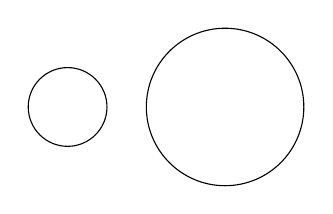
\begin{tikzpicture}[xkcd]
    \draw (0,0) circle (0.5cm);
    \draw (2,0) circle (1cm);
\end{tikzpicture}
\end{center}

\begin{center}
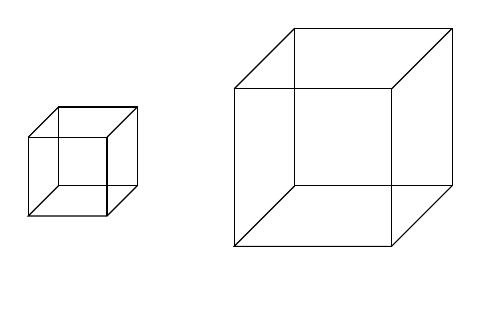
\begin{tikzpicture}[xkcd]
    \draw (0,0,0) -- (1,0,0) -- (1,1,0) -- (0,1,0) -- cycle;
    \draw (0,0,0) -- (0,0,1) -- (1,0,1) -- (1,0,0);
    \draw (1,0,1) -- (1,1,1) -- (0,1,1) -- (0,0,1);
    \draw (1,1,0) -- (1,1,1);
    \draw (0,1,0) -- (0,1,1);
    \node at (0.5,-0.5,0.5) {};

    \begin{scope}[xshift=3cm,scale=2]
    \draw (0,0,0) -- (1,0,0) -- (1,1,0) -- (0,1,0) -- cycle;
    \draw (0,0,0) -- (0,0,1) -- (1,0,1) -- (1,0,0);
    \draw (1,0,1) -- (1,1,1) -- (0,1,1) -- (0,0,1);
    \draw (1,1,0) -- (1,1,1);
    \draw (0,1,0) -- (0,1,1);
    \node at (0.5,-0.5,0.5) {};
    \end{scope}
\end{tikzpicture}
\end{center}

Discuss how your estimates compare to the actual ratios. Did you notice that it became harder to estimate accurately for areas and volumes?

\newpage

\begin{minipage}{\textwidth}
    {\bf Question 2: Histograms}

    \begin{enumerate}
        \item Draw a histogram representing the number of hours people spend watching Game of Thrones per week. Use the following data:

        \begin{center}
            \begin{tabular}{|c|c|}
                \hline
                Hours per week & Number of people \\
                \hline
                $(0,2]$ & 15 \\
                $(2,4]$ & 25 \\
                $(4,6]$ & 35 \\
                $(6,8]$ & 20 \\
                $(8,10]$ & 5 \\
                \hline
            \end{tabular}
        \end{center}

        Use equal bin sizes and label your axes appropriately.

        \item Now, draw another histogram using the same data but with varying bin sizes:
        \begin{center}
            \begin{tabular}{|c|c|}
                \hline
                Hours per week & Number of people \\
                \hline
                $(0,2]$ & 15 \\
                $(2,4]$ & 40 \\
                $(4,8]$ & 45 \\
                $(8,16]$ & 30 \\
                $(16,32]$ & 20 \\
                \hline
            \end{tabular}
        \end{center}
        How does this change the appearance of the distribution?
    \end{enumerate}
\end{minipage}

\newpage

{\bf Question 3:} Consider the following linear and logarithmic scales:
Mark the position of 5 and 25 on the logarithmic scale.

\begin{center}
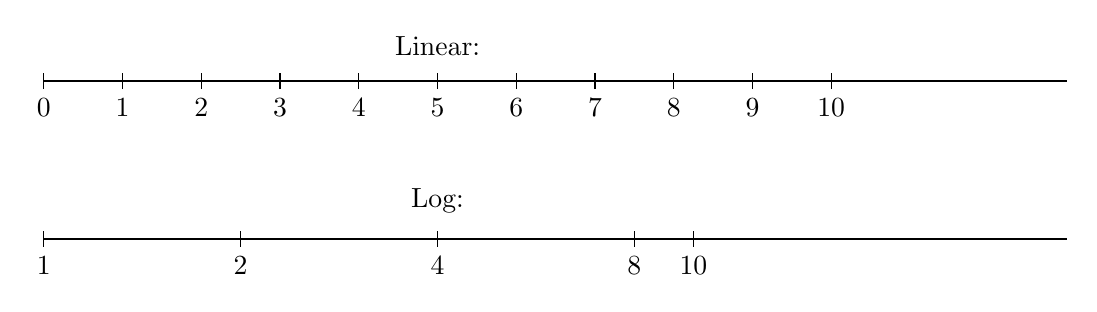
\begin{tikzpicture}
    % Linear scale
    \draw[thick] (0,2) -- (13,2);
    \foreach \x in {0,1,...,10} {
        \draw (\x,1.9) -- (\x,2.1);
        \node[below] at (\x,1.9) {\x};
    }
    \node[above] at (5,2.2) {Linear:};

    % Logarithmic scale
    \draw[thick] (0,0) -- (13,0);
    \foreach \x/\label in {0/1,1/2,2/4,3/8,3.3/10} {
        \draw (\x*2.5, -0.1) -- (\x*2.5, 0.1);
        \node[below] at (\x*2.5, -0.1) {\label};
    }
    \node[above] at (5,0.2) {Log:};
\end{tikzpicture}
\end{center}


{\bf Question 4:} Draw a histogram using a logarithmic scale for the x-axis (hours watched) using the data from Question 2.2.

\newpage

{\bf Question 5:}

\begin{tcolorbox}
The Cumulative Distribution Function (CDF) of a random variable \(X\) is defined as:
\[
F(x) = P(X \leq x)
\]
It represents the fraction of data points that are less than or equal to \(x\).
The Complementary Cumulative Distribution Function (CCDF) is defined as:
\[
\bar{F}(x) = P(X > x) = 1 - F(x)
\]
It represents the the fraction of data points that are greater than \(x\).
\end{tcolorbox}


1. Draw the CDF and CCDF of the following data in linear scale.

\begin{center}
\{0, 1, 2, 5, 3, 7, 1, 9, 4, 6, 2, 8, 5, 10, 5, 7, 4, 8, 8, 1\}
\end{center}

2. Draw the CDF and CCDF of the following data in logarithmic scale (both x and y axes).

\begin{center}
\{1, 2, 4, 8, 16, 32, 64, 128, 256, 512, 1024, 2048, 1, 2, 4, 8, 16, 32, 256, 1, 2, 4, 32, 64, 1\}
\end{center}



\end{document}
